\chapter{Aerodynamic Analysis}  \label{cp:aero}

% Briefly introduce the topic/purpose of this chapter, what information can be found in this chapter, and the key findings.
% Patricia


In this wind tunnel analysis, we will be discusing results obtained from the wind tunnel (experimental) analysis and the results obtained through CFD and how they differ from each other at varying the angles of attack.
The effects of the aerodynamic forces acting on an airfoil, specifically focusing on lift and drag behavior. Everything discussed below will be supported by graphs for the experimental analysis (wind tunnel), CFD analysis and Comparison between both. 
For lift, we observed that as the angle of attack increased, lift increased steadily due to the growing pressure difference between the upper and lower surfaces of the airfoil. This trend continued until reaching a critical angle of attack, after which lift began to decrease as flow separation occurred, leading to stall.

For drag, we noted that it remained relatively low at small angles of attack but began to rise significantly as the angle increased. This increase became especially noticeable near and beyond the stall angle, where the separated flow created more turbulence and pressure drag on the airfoil.

The comparison between the drag coefficient (Cd) from CFD and experimental wind tunnel data revealed notable differences in drag behavior. From 0° to 14° angle of attack, the CFD results predicted higher drag values than the wind tunnel, suggesting that the CFD model might have overestimated drag in this range, possibly due to limitations in turbulence modeling or flow characteristics.

However, at angles beyond 14°, the experimental data showed a sharp spike in drag, surpassing the CFD predictions. This spike likely represents the onset of flow separation and stall, where the experimental setup captured a more pronounced increase in drag due to turbulence and wake formation. The CFD model, on the other hand, struggled to fully replicate these phenomena, highlighting discrepancies in accurately simulating the transition to stall.

%   Tommy
\newpage

\section{Experimental Data}

\begin{figure}[htpb]
    \centering
    \includesvg[width=\linewidth]{figures/aero_data/experimental_cl.svg}
    \caption[The experimental \gls{C_L} versus \acrshort{aoa}]{The experimental coefficient of lift (\gls{C_L}) versus the \acrshort{aoa}.}
    \label{fig:experimental_cl}
\end{figure}


% Patricia

%\begin{figure}[htbp]
    %\centering
   % 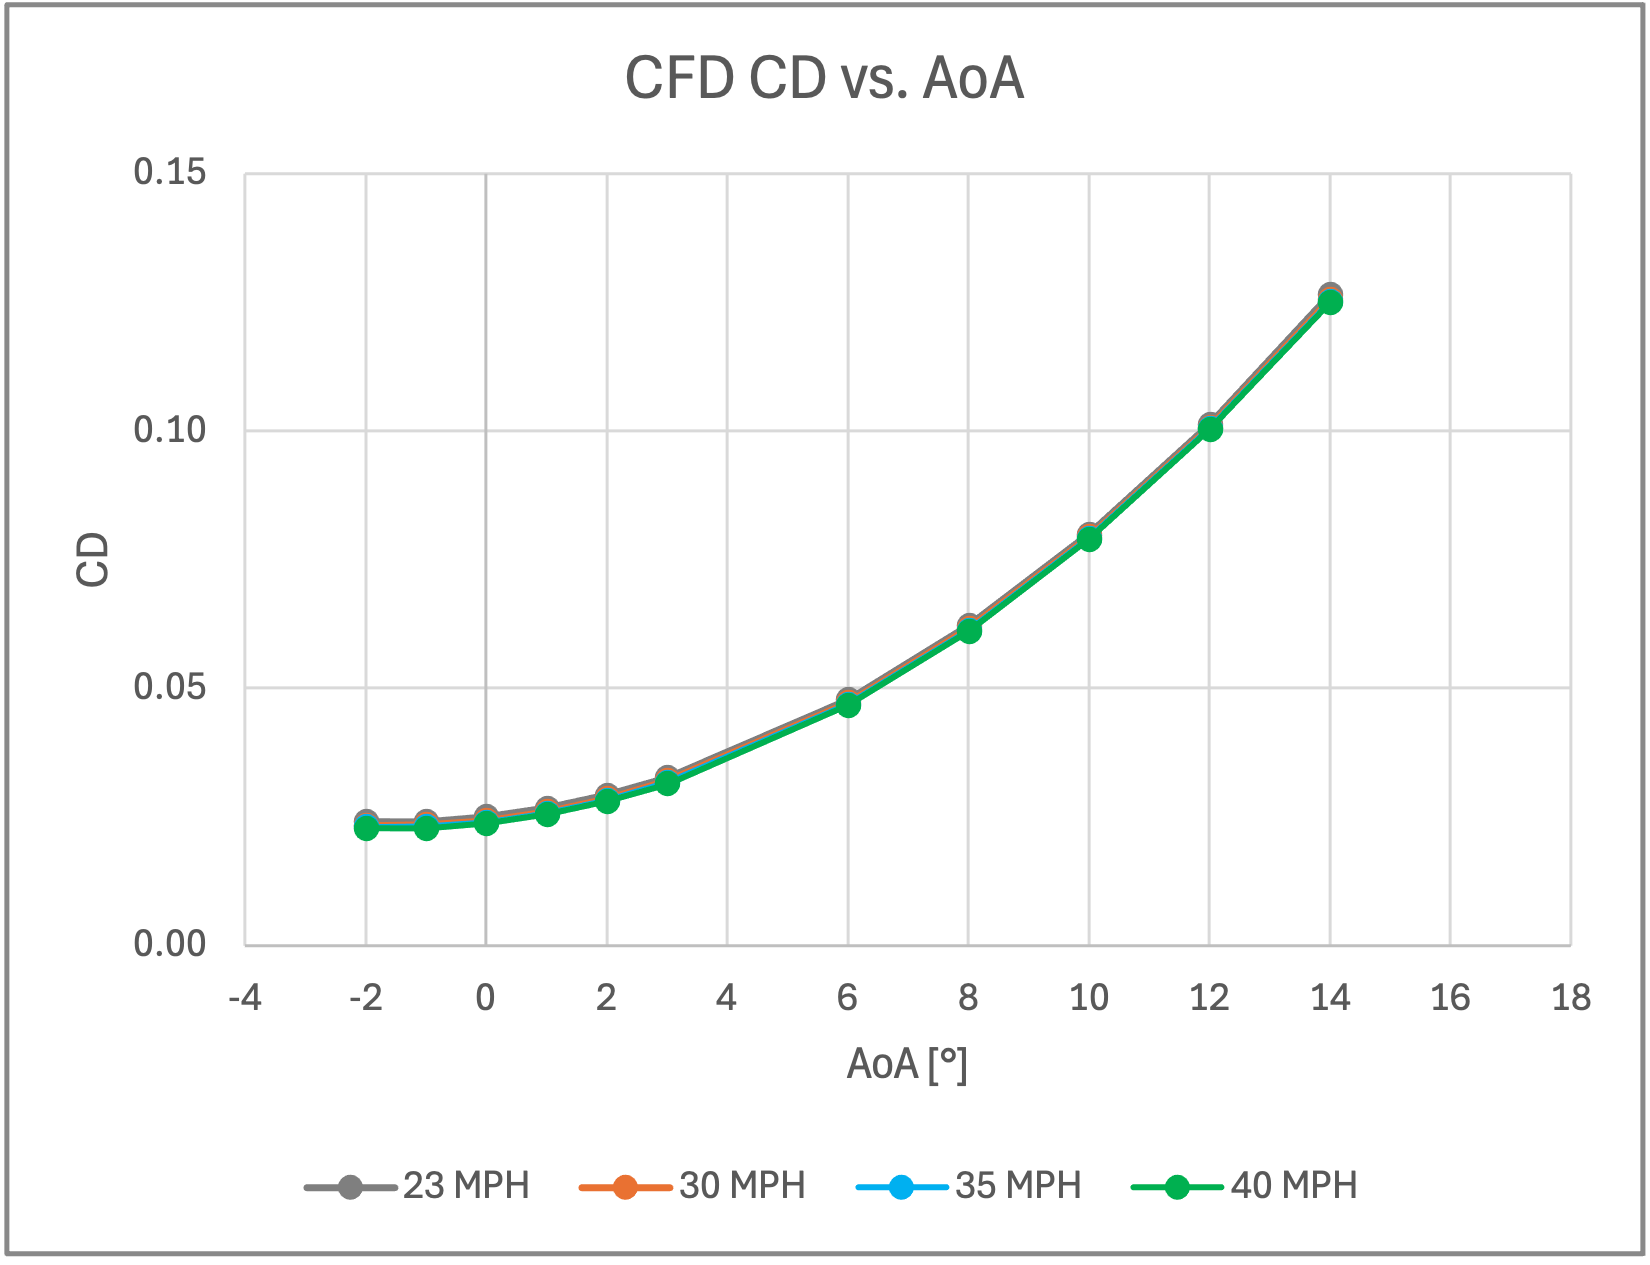
\includegraphics[width=\linewidth]{figures/aero_data/CFDCDvsAoA.png}
    %\caption[The experimental \gls{C_D} versus \acrshort{aoa}]{The CFD data of lift coefficient  (\gls{C_L}) versus the \acrshort{aoa}}
    %\label{fig:experimental_cl}
%\end{figure}%
